%!TEX program = xelatex
%%%%%%%%%%%%%%%%%%%%%%%这是导言部分的开始%%%%%%%%

%========= 导言部分声明文档的类型=================
\documentclass{article}

%=========导言部分可可以加载宏包=================
\usepackage{amsmath}                % 数学公式排版宏包
\usepackage{amssymb}                % 数学符号命令宏包
\usepackage{amsthm}                 % 数学定理宏包
\usepackage[UTF8]{ctex}             % 中文输入宏包
\usepackage[a4paper]{geometry}      % 页面设置宏包
\usepackage{setspace}               % 行间距宏包
\usepackage{graphicx}               % 图片宏包
\usepackage{listings}               % 代码宏包
\usepackage{color}					% 颜色宏包
\usepackage{xcolor}                 % 颜色处理宏包
\usepackage{float}                  % 浮动对象式样宏包
\usepackage{fontspec}
\usepackage{enumerate}				% 列举编号包

%=========页面设置==============================
\geometry{left=1cm,right=1cm,top=1cm,bottom=2cm}
\onehalfspacing
\setlength\parindent{0em}

%=========代码格式设置============================
\definecolor{dkgreen}{rgb}{0,0.6,0}
\definecolor{gray}{rgb}{0.5,0.5,0.5}
\definecolor{mauve}{rgb}{0.58,0,0.82}
% \setmonofont{Consolas}
\lstset{
	numbers = left, 	
	numberstyle = \color{gray}, 
	keywordstyle = \color{blue},
	commentstyle = \color{dkgreen}, 
	stringstyle = \color{mauve},
	basicstyle = \ttfamily,
	breaklines = true,
	frame = shadowbox, % 阴影效果
	rulesepcolor = \color{ red!20!green!20!blue!20} ,
	escapeinside = ``, % 英文分号中可写入中文
	xleftmargin = 2em,xrightmargin=2em, aboveskip=1em,
	framexleftmargin = 2em
} 

%=========导言部分可以定义标题信息===============
\title{组会报告}
\author{徐益}
\date{\today}
%%%%%%%%%%%%%%%%%%%%%%%这是导言部分的结束%%%%%%%%%

%%%%%%%%%%%%%%%%%%%%%%%这是正文部分的开始%%%%%%%%%
\begin{document}

%=========生成标题================================
\maketitle

%=========开始正文的输入==========================

%===========第一节=================
\section{工作内容} 
1. 学习自适应调制编码相关内容;

2. 测试5GNR自适应调制编码各CQI门限SNR。

3. 搭建基于C的5GNR自适应调制编码参数测试平台。

%===========第二节=================
\section{学习自适应调制编码相关内容}
\subsection{LTE下行链路自适应传输系统}
\begin{figure}[H]
	\centering
	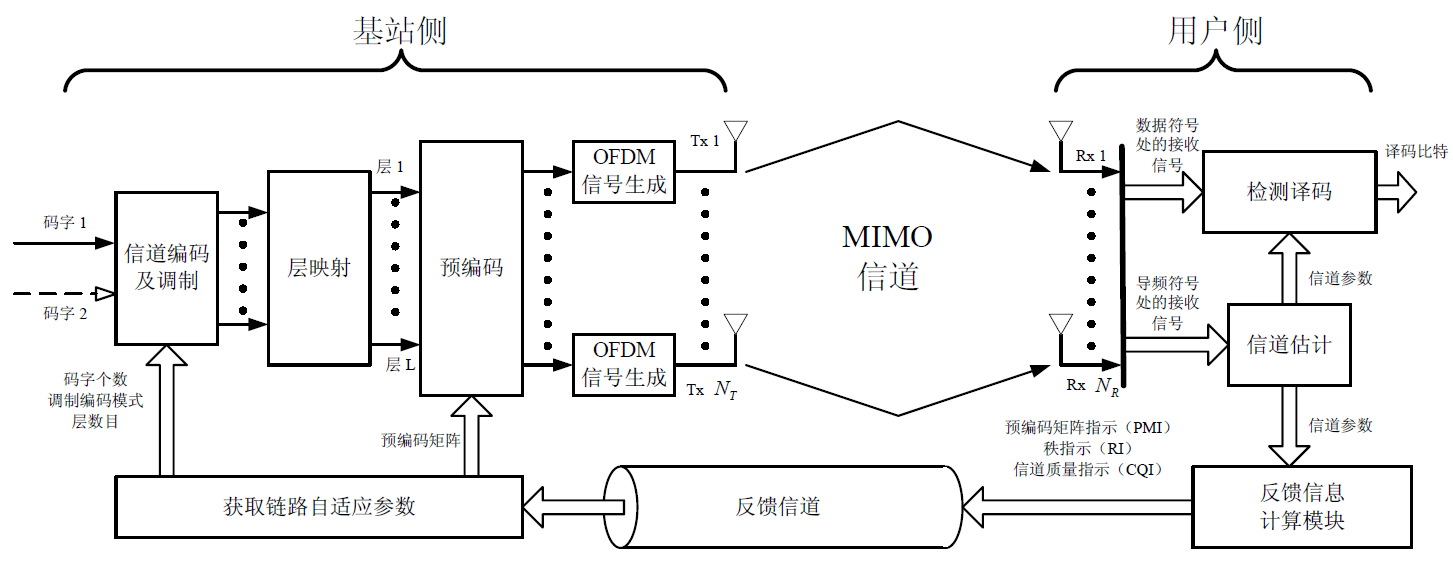
\includegraphics[width = \textwidth]{system.png}
	\caption{MAC-LTE下行链路自适应传输系统框图}
\end{figure}
\subsection{自适应调制编码}
\subsubsection{获得各CQI值对应的门限值}
在AWGN信道中的各个CWER-SNR曲线上,读出各个MCS在CWER=0.1处的门限,用$SNR_{th,index}$表示,其中$index=0,1,...,31$。
\subsubsection{计算各CQI对应的等效信噪比}
首先根据当前信道矩阵和预编码矩阵算出各个资源上的信干噪比$SINR_{k,n,l}$,再根据式(1)的EESM映射方法,
得到不同CQI对应的等效信噪比,用$SNR_{eff,index}$表示,其中$index=0,1,...,31$。
\begin{equation}
	SNR_{eff}=-\beta\ln(\frac{1}{LKN}\sum_{l=0}^{L-1}\sum_{k=0}^{K-1}\sum_{n=0}^{N-1}exp(-\frac{SINR_{k,n,l}}{\beta}))
\end{equation}
其中$L$是层数,$K$是子载波个数,$N$是OFDM符号数,$\beta$是修正因子,获取需要两个步骤:\\
第一,生成足够多的信道实现以确保能够遍历所有的信道状态,在每个信道实现以保证能够遍历所有的信道状态,
在每个信道下通过链路级仿真得到相应的BLER,用$BLER_i$表示,$i=1,...,N_C$,$N_C$为信道实现的个数,
查找AWGN信道下与该MCS对应的BLER-SNR曲线得到$BLER_i$相应的等效信噪比,用$SNR_{AWGN,i}$表示。\\
第二,对每个信道实现,利用式(1)计算出EESM预测得到的等效信噪比,用$SNR_{EESM,i}$表示。
将EESM得到的等效信噪比与实际仿真得到的信噪比进行比较,为使EESM方法有准确的近似,最优的$\beta$
应使两者的均方误差最小:
\begin{equation}
	\beta_{opt}=\mathrm{arg}\min_{\beta}{ \sum_{i=0}^{N_C}|{SNR_{AWGN,i}}-SNR_{EESM,i}|^2 }
\end{equation}
\subsubsection{确定CQI}
对应比较第一步得到的$SNR_{th,index}$和第二步得到的$SNR_{eff,index}$,UE反馈的CQI为使得
$SNR_{eff,index}$超过$SNR_{th,index}$最大的$index$,即
\begin{equation}
    CQI=\mathrm{arg}\max_{index\in\{0,...,31\}} SNR_{eff,index}\geq SNR_{th,index}
\end{equation}

%===========第三节=================
\section{测试5GNR自适应调制编码各CQI门限SNR}
\begin{figure}[H]
	\centering
	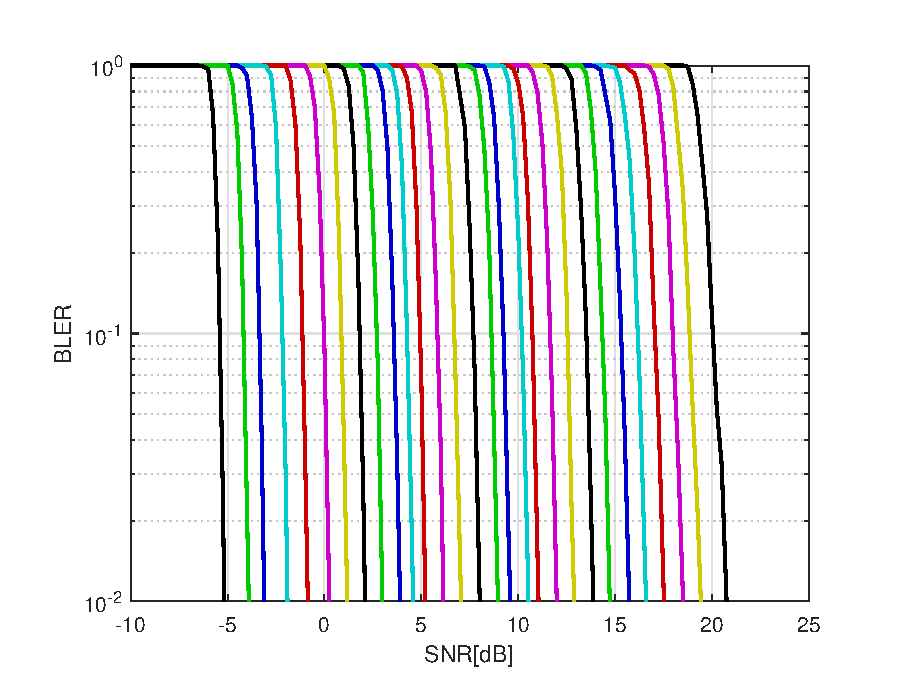
\includegraphics[width = .8\textwidth]{bler.eps}
	\caption{AWGN信道下各CQI的BLER-SNR曲线}
\end{figure}

\begin{table}[H]
	\caption{不同CQI的门限SNR值}
	\centering
	\begin{tabular}{|l|l|l|l|l|l|l|}% 通过添加 | 来表示是否需要绘制竖线
		\hline  % 在表格最上方绘制横线
		CQI		& Q		& R		& $SNR_{th}$(dB)    \\
		\hline
		0		& 2		& 120	& -5.41 \\
		\hline
		1		& 2		& 157	& -4.18 \\
		\hline
		2		& 2		& 193	& -3.36 \\
		\hline
		3		& 2		& 251	& -2.18 \\
		\hline
		4		& 2		& 308	& -1.14 \\
		\hline
		5		& 2		& 379	& -0.03 \\
		\hline
		6		& 2		& 449	& 0.87  \\
		\hline
		7		& 2		& 586	& 1.81  \\
		\hline
		8		& 2		& 602	& 2.70  \\
		\hline
		9		& 2		& 679	& 3.57  \\
		\hline
		10		& 4		& 340	& 4.26  \\
		\hline
		11		& 4		& 378	& 4.93  \\
		\hline
		12		& 4		& 434	& 5.83  \\
		\hline
		13		& 4		& 490	& 6.70  \\
		\hline
		14		& 4		& 553	& 7.68  \\
		\hline
		15		& 4		& 616	& 8.62 \\
		\hline
		16		& 4		& 658	& 9.24 \\
		\hline
		17		& 6		& 438	& 10.18 \\
		\hline
		18		& 6		& 466	& 10.73 \\
		\hline
		19		& 6		& 517	& 11.64 \\
		\hline
		20		& 6		& 567	& 12.54 \\
		\hline
		21		& 6		& 616	& 13.52 \\
		\hline
		22		& 6		& 666	& 14.34 \\
		\hline
		23		& 6		& 719	& 15.31 \\
		\hline
		24		& 6		& 772	& 16.17 \\
		\hline
		25		& 6		& 822	& 17.05 \\
		\hline
		26		& 6		& 873	& 17.97 \\
		\hline
		27		& 6		& 910	& 18.84 \\
		\hline
		28		& 6		& 948	& 20.04 \\
		\hline  % 在表格最下方绘制横线
	\end{tabular}
\end{table}

%===========第四节=================
\section{搭建基于C的5GNR自适应调制编码参数测试平台}
问题:
\begin{figure}[H]
	\centering
	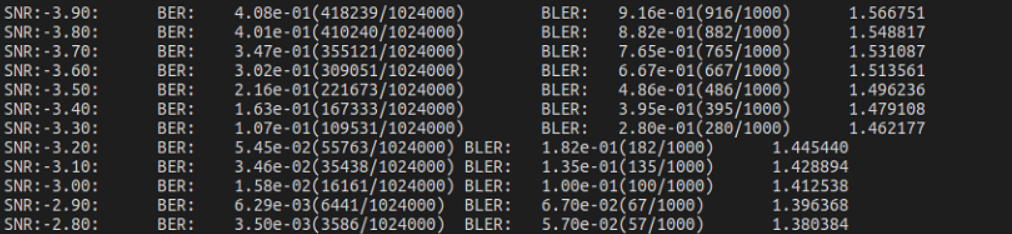
\includegraphics[width = \textwidth]{problem.png}
	\caption{C平台上测试SNR门限信噪比的问题}
\end{figure}

%===========第五节=================
% \section{有PRACH情况下的资源分配问题}
% \begin{figure}[H]
% 	\centering
% 	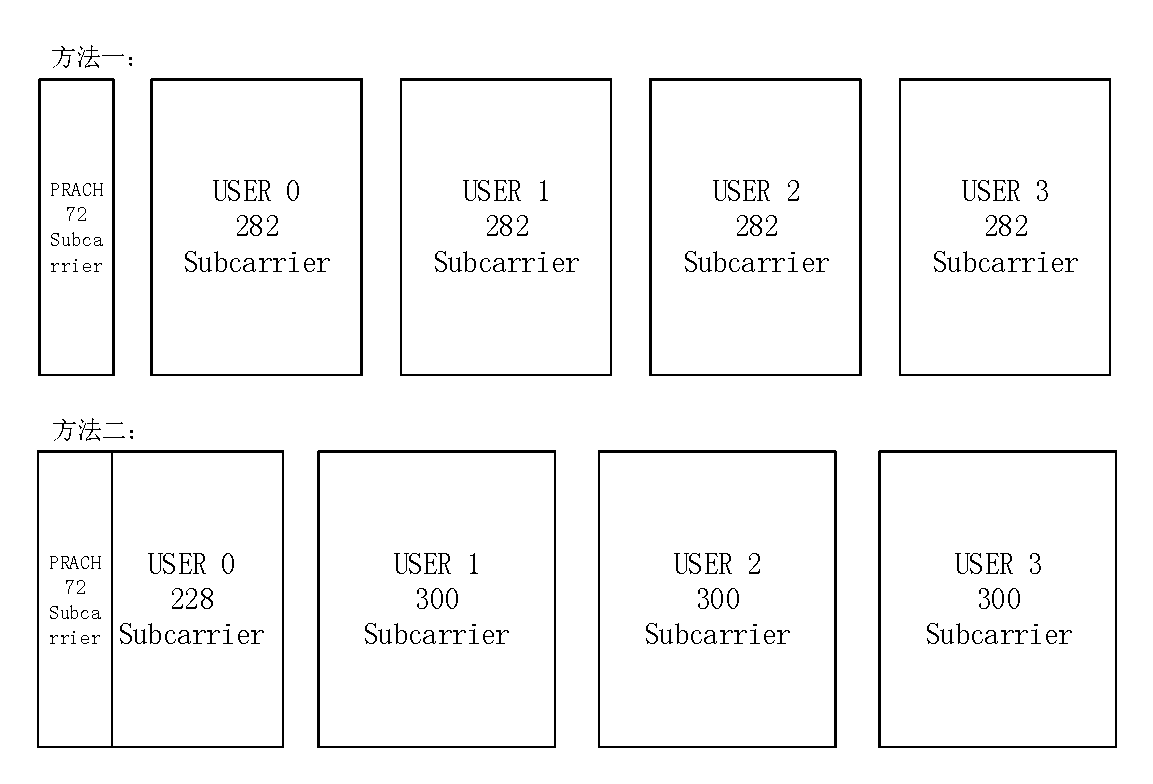
\includegraphics[width = \textwidth]{ques.pdf}
% 	\caption{两种方案}
% \end{figure}

%===========下周计划=================
% \section{下阶段计划}
% 1. 完善单线程系统(修复Bug)

\end{document}
%%%%%%%%%%%%%%%%%%%%%%%这是正文部分的结束%%%%%%%%%%%%